\chapter{Model}
\label{Chapter3}
This chapter aims to totally describe the proposed model. Before going into the description details, Section \ref{challenge} tries to frame the difficulties that the model has to deal with, in trying to solve a classification task of the one described in Section \ref{classification}. These observations aim to provide a preliminary justification and comprehension of the reasons behind specific choices.

\section{What is the challenge?}
\label{challenge}
\begin{table}[H]
  \centering
  \caption{Performance of some configurations of a simple Neural-Symbolic model. All accuracy values are in percentage and approximated to the second digit after the decimal place.}
  \label{tab:simple-model}
  \scriptsize
  \begin{tabular}{ccccccrr}
    \toprule
    depth		& distributions 			& splits 		& sums 				& dropout input 		& dropout sums 			& valid acc 			& test acc\\
    \midrule
    1			& 10						& 9 			& 10 				& 0.5 					& 0.75 					& 95.03 				& 94.88\\
	1			& 10						& 9 			& 10 				& 0.5 					& 1 					& 27.55 				& 26.78\\
	1			& 10						& 9 			& 10 				& 0.75 					& 1 					& 97 .01				& 96.11\\
	\textbf{1}	& \textbf{10}				& \textbf{9} 	& \textbf{10} 		& \textbf{0.25} 		& \textbf{0.25} 		& \textbf{6.12} 		& \textbf{5.74}\\
	1			& 10						& 9 			& 10 				& 0.50 					& 0.25 					& 94.51 				& 94.65\\
	1			& 10						& 9 			& 10 				& 0.25 					& 0.5 					& 94.48 				& 94.08\\
	1			& 33						& 40 			& 10 				& 0.25 					& 0.5 					& 92.92 				& 92.75\\
	1			& 33						& 40 			& 10 				& 0.5 					& 0.25 					& 59.13 				& 58.93\\
	1			& 33						& 40 			& 10 				& 0.75 					& 0.25 					& 84.22 				& 84.75\\
	1			& 33						& 40 			& 10 				& 0.25 					& 1 					& 19.83 				& 19.96\\
    1			& 33						& 40 			& 10 				& 0.5 					& 1 					& 96.27 				& 96.24\\
	1			& 33						& 40 			& 10 				& 0.5 					& 0.5 					& 96.53 				& 96.16\\
    \bottomrule
  \end{tabular}
\end{table}
Table \ref{tab:simple-model} shows the performance of some configurations (for brevity) of a very simple Neural-Symbolic model, whose subsymbolic module training is based on the most probable abduction among the ones suggested by the symbolic module; the task consists in learning to classify digits from 0 to 9, knowing the sum of $n$ pairs of them. For the moment, further details about the classification task and the model under consideration are intentionally omitted, in order to focus the attention on the findings. Looking at the results, a significant variance in terms of accuracy is evident among the tested configurations. In order to investigate this anomalous behaviour and to understand if such a variance depends on the specific configuration (i.e. on the the sub-symbolic hyperparameters) or not, the configuration highlighted in bold in Table \ref{tab:simple-model} has been runned multiple times.

\begin{table}[H]
  \caption{Multiple runs of configuration higlighted in bold in Table \ref{tab:simple-model}. Reported values refer to accuracy computed on validation set (in percentage).}
  \label{tab:multiple-run}
  \centering
  \renewcommand{\arraystretch}{0.8}
  \begin{tabular}{cccc}  
    %\toprule
						& \textbf{run 1} & \textbf{run 2} & \textbf{run 3} \\
	\hline
	\textbf{epoch 0}	& 14.98 			& 47.21 		& 33.91  \\
	\hline
	\textbf{epoch 30}	& 11.65 			& 70.85 		& 52.15  \\
	\hline
	\textbf{epoch 50}	& 10.32 			& 90.12 		& 78.92  \\
	\hline
	\textbf{epoch 100} 	& 12.79				& 93.22 		& 88.34  \\
	\bottomrule
	\end{tabular}
\end{table}
Results of Table \ref{tab:multiple-run} clearly show that the variance in the model performance does not depend on the considered combination of hyperparameters, since multiple runs of the same configuration bring to very different values in terms of accuracy. With the aim of furtherly investigate this attitude, Tables \ref{tab:confusion-matrix-1}, \ref{tab:confusion-matrix-2} and \ref{tab:confusion-matrix-3} show the confusion matrices of the first epoch of such runs, calculated taking into account the real labels of the considered digits and the labels selected by the sub-symbolic module among the ones suggested by symbolic one. In particular, since each value has been obtained dividing the observed frequency by the correspondent row sum, the element in position $(i,j)$ indicates the ratio with which the $i-th$ digit has been labeled as the $j-th$ one by the model (the reverse observation can NOT be done). These matrices point out that the strong variance in terms of accuracy lies in the variability with whom the examples are labelled on the basis of the symbolic module abductions and the subsymbolic module probabilities. Since the initialization of the subsymbolic module is random and since the most probable abduction is chosen according to the probability computed by the SPN, selected abductions to train the model are random likewise. Therefore, since the model has no way to understand if it is going well or not, the first taken direction significantly influences all the training procedure. Essentially, the model goodness depends on chance: only if the first abduced labels are (by chance) correct, the model performance are quite good. It is clear that this behaviour can't be considered as a real learning. Furthermore, the more the task becomes difficult (in terms of the number of possible abductions), the more the chance of randomly abducing the correct labels decreases. 

The considerations made up to now emphasise that, since the abduction is not a reasoning process that returns always true facts and especially because the initialization of the subsymbolic model is randomic, we need to try to force the model not to learn from abductions it is not sufficently sure of, trying to guide somehow it towards the real most probable ones. All the choices explained in the following section are oriented in this perspective.

\begin{table}[H]
  \caption{Confusion matrix between real labels (row) and abduced labels (column) for run 1 of Table \ref{tab:multiple-run}. Each reported value has been obtained dividing the observed frequency by the correspondent row sum and approximated to the second digit after the decimal place. Accuracy on validation set: 14.98\%}
  \label{tab:confusion-matrix-1}
  \centering
  \begin{tabular}{ccccccccccc}  
    %\toprule
						& \textbf{0} & \textbf{1} & \textbf{2} & \textbf{3} & \textbf{4} & \textbf{5} & \textbf{6} & \textbf{7} & \textbf{8} & \textbf{9}\\
	\hline
	\textbf{0}			& \textbf{0.27} & 0.17 & 0.27 & 0.06 & 0.06 & 0.04 & 0.03 & 0.09 & 0.00 & 0.00  \\
	\hline
	\textbf{1}			& 0.14 & \textbf{0.21} & 0.17 & 0.08 & 0.14 & 0.25 & 0.00 & 0.00 & 0.00 & 0.00  \\
	\hline
	\textbf{2}			& 0.14 & 0.11 & \textbf{0.26} & 0.09 & 0.12 & 0.13 & 0.03 & 0.06 & 0.05 & 0.02  \\
	\hline
	\textbf{3} 			& 0.06 & 0.09 & 0.23 & \textbf{0.09} & 0.09 & 0.25 & 0.06 & 0.06 & 0.05 & 0.02  \\
	\hline
	\textbf{4} 			& 0.04 & 0.06 & 0.17 & 0.09 & \textbf{0.09} & 0.31 & 0.12 & 0.06 & 0.05 & 0.02  \\
	\hline
	\textbf{5} 			& 0.06 & 0.06 & 0.08 & 0.07 & 0.13 & \textbf{0.26} & 0.11 & 0.09 & 0.09 & 0.05  \\
	\hline
	\textbf{6} 			& 0.03 & 0.02 & 0.10 & 0.04 & 0.16 & 0.20 & \textbf{0.16} & 0.19 & 0.06 & 0.05  \\
	\hline
	\textbf{7} 			& 0.02 & 0.01 & 0.05 & 0.04 & 0.08 & 0.27 & 0.16 & \textbf{0.10} & 0.16 & 0.11  \\
	\hline
	\textbf{8} 			& 0.00 & 0.03 & 0.05 & 0.02 & 0.09 & 0.15 & 0.13 & 0.10 & \textbf{0.31} & 0.11  \\
	\hline
	\textbf{9} 			& 0.00 & 0.00 & 0.06 & 0.02 & 0.03 & 0.20 & 0.13 & 0.09 & 0.22 & \textbf{0.25}  \\
	\bottomrule
	\end{tabular}
\end{table}

\begin{table}[H]
  \caption{Confusion matrix between real labels (row) and abduced labels (column) for run 2 of Table \ref{tab:multiple-run}. Each reported value has been obtained dividing the observed frequency by the correspondent row sum and approximated to the second digit after the decimal place. Accuracy on validation set: 47.21\%}
  \label{tab:confusion-matrix-2}
  \centering
  \begin{tabular}{ccccccccccc}  
    %\toprule
						& \textbf{0} & \textbf{1} & \textbf{2} & \textbf{3} & \textbf{4} & \textbf{5} & \textbf{6} & \textbf{7} & \textbf{8} & \textbf{9}\\
	\hline
	\textbf{0}			& \textbf{0.39} & 0.16 & 0.18 & 0.08 & 0.05 & 0.05 & 0.05 & 0.03 & 0.01 & 0.01  \\
	\hline
	\textbf{1}			& 0.09 & \textbf{0.41} & 0.11 & 0.18 & 0.06 & 0.01 & 0.01 & 0.11 & 0.02 & 0.00  \\
	\hline
	\textbf{2}			& 0.12 & 0.13 & \textbf{0.25} & 0.17 & 0.1  & 0.08 & 0.05 & 0.04 & 0.04 & 0.02  \\
	\hline
	\textbf{3} 			& 0.08 & 0.10 & 0.13 & \textbf{0.29} & 0.12 & 0.07 & 0.08 & 0.04 & 0.04 & 0.05  \\
	\hline
	\textbf{4} 			& 0.03 & 0.11 & 0.10 & 0.15 & \textbf{0.15} & 0.05 & 0.12 & 0.23 & 0.03 & 0.03  \\
	\hline
	\textbf{5} 			& 0.03 & 0.04 & 0.10 & 0.16 & 0.11 & \textbf{0.12} & 0.16 & 0.18 & 0.04 & 0.06  \\
	\hline
	\textbf{6} 			& 0.04 & 0.03 & 0.04 & 0.11 & 0.06 & 0.09 & \textbf{0.37} & 0.12 & 0.07 & 0.06  \\
	\hline
	\textbf{7} 			& 0.01 & 0.05 & 0.03 & 0.04 & 0.07 & 0.04 & 0.07 & \textbf{0.47} & 0.17 & 0.05  \\
	\hline
	\textbf{8} 			& 0.00 & 0.02 & 0.09 & 0.04 & 0.05 & 0.07 & 0.14 & 0.21 & \textbf{0.25} & 0.14  \\
	\hline
	\textbf{9} 			& 0.01 & 0.00 & 0.04 & 0.08 & 0.03 & 0.04 & 0.11 & 0.26 & 0.23 & \textbf{0.21}  \\
	\bottomrule
	\end{tabular}
\end{table}

\begin{table}[H]
  \caption{Confusion matrix between real labels (row) and abduced labels (column) for run 3 of Table \ref{tab:multiple-run}. Each reported value has been obtained dividing the observed frequency by the correspondent row sum and approximated to the second digit after the decimal place. Accuracy on validation set: 33.91\%}
  \label{tab:confusion-matrix-3}
  \centering
  \begin{tabular}{ccccccccccc}  
    %\toprule
						& \textbf{0} & \textbf{1} & \textbf{2} & \textbf{3} & \textbf{4} & \textbf{5} & \textbf{6} & \textbf{7} & \textbf{8} & \textbf{9}\\
	\hline
	\textbf{0}			& \textbf{0.39} & 0.12 & 0.22 & 0.08 & 0.03 & 0.03 & 0.10 & 0.01 & 0.00 & 0.02  \\
	\hline
	\textbf{1}			& 0.10 & \textbf{0.37} & 0.06 & 0.23 & 0.07 & 0.04 & 0.01 & 0.11 & 0.01 & 0.00  \\
	\hline
	\textbf{2}			& 0.14 & 0.07 & \textbf{0.33} & 0.14 & 0.08 & 0.04 & 0.10 & 0.03 & 0.04 & 0.03  \\
	\hline
	\textbf{3} 			& 0.06 & 0.12 & 0.06 & \textbf{0.41} & 0.08 & 0.10 & 0.03 & 0.05 & 0.04 & 0.05  \\
	\hline
	\textbf{4} 			& 0.07 & 0.07 & 0.09 & 0.14 & \textbf{0.19} & 0.10 & 0.11 & 0.19 & 0.03 & 0.03  \\
	\hline
	\textbf{5} 			& 0.04 & 0.04 & 0.07 & 0.18 & 0.07 & \textbf{0.22} & 0.08 & 0.17 & 0.05 & 0.08  \\
	\hline
	\textbf{6} 			& 0.07 & 0.01 & 0.04 & 0.09 & 0.05 & 0.05 & \textbf{0.44} & 0.11 & 0.07 & 0.07  \\
	\hline
	\textbf{7} 			& 0.01 & 0.07 & 0.02 & 0.05 & 0.06 & 0.06 & 0.04 & \textbf{0.54} & 0.07 & 0.08  \\
	\hline
	\textbf{8} 			& 0.01 & 0.02 & 0.08 & 0.06 & 0.05 & 0.10 & 0.11 & 0.25 & \textbf{0.17} & 0.15  \\
	\hline
	\textbf{9} 			& 0.02 & 0.00 & 0.02 & 0.09 & 0.02 & 0.07 & 0.08 & 0.34 & 0.13 & \textbf{0.23}  \\
	\bottomrule
	\end{tabular}
\end{table}

\section{Architecture and features}
\label{arch-and-feat}
Figure \ref{fig:architecture} shows the general architecture of the implemented model. Essentially:

\begin{itemize}
	\item the symbolic module, containing the domain knowledge, takes in input the aggregate information (elements of $\mathit{F}$ deriving from the application of function $\mathit{f}$, see Section \ref{classification}) related to the observations and returns all the possible abductions;
	\item the sub-symbolic module, which consists in a Random And Tensorized SPN (RAT-SPN), receives such explanations together with the observations and, on the basis of the most probable ones (i.e., abductions), performs the training process. Note that RAT-SPN is unuware about $\mathit{f}$, it just works on observations and labels abduced by symbolic module.
\end{itemize}
In the following, we describe in detail the implemented features (in the figure, red numbers from 1 to 4) that allow the final model to perform better than the one described in Section \ref{challenge}.

\begin{figure}[H]
\caption{Model architecture.}
\label{fig:architecture}
\centering
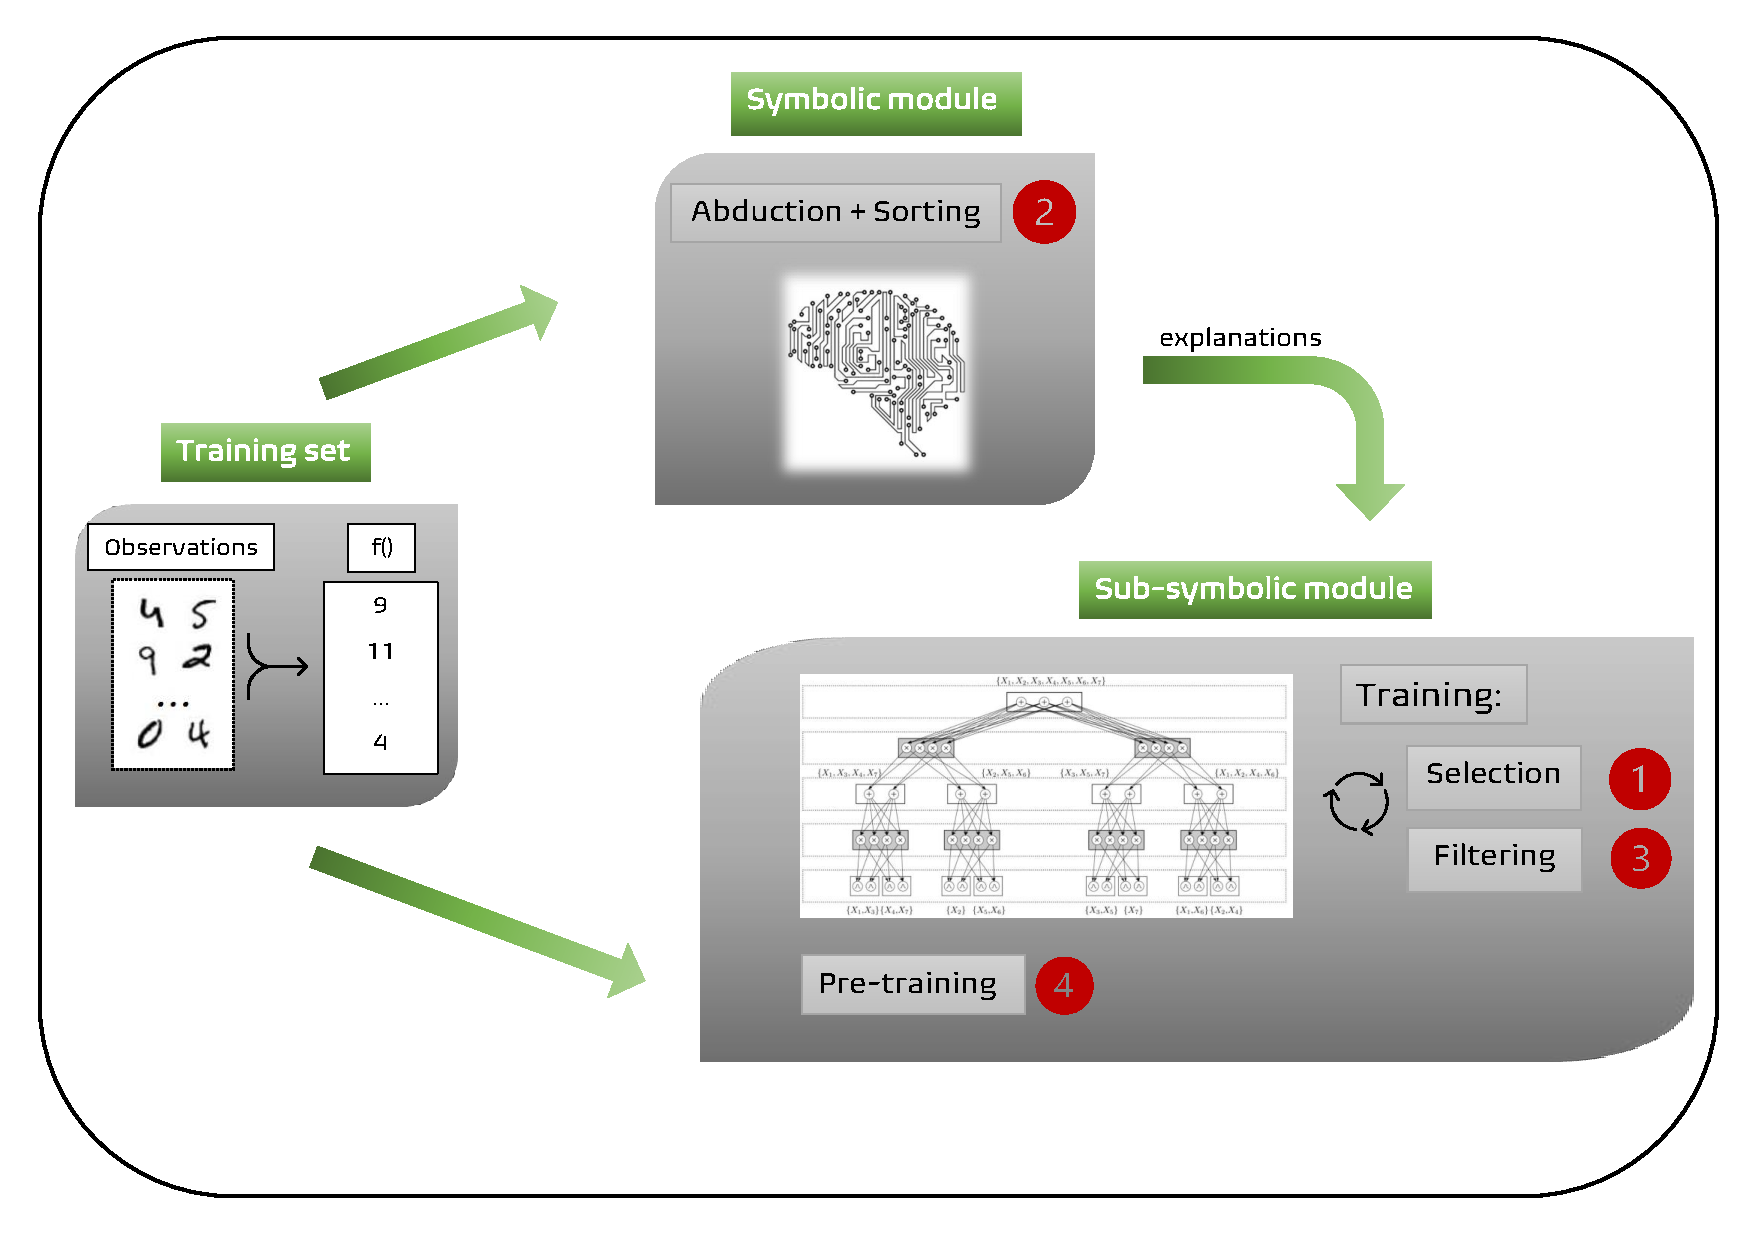
\includegraphics[scale=0.45]{Figures/architecture.pdf}
\end{figure}

\subsection{Abduction selection}
\label{abd-selection}
Since the function $\mathit{f}$ is not injective, the symbolic module suggests more than one possible abduction for each observation of the training set. The first key-point is to decide how to select the most suitable (ideally the correct) one in order to perform the training process. Let:

\begin{itemize}
	\item $\mathit{A}$ be the set of abductions returned by symbolic module for observations $\mathbf{x}_r,...,\mathbf{x}_{r+m} \in \mathit{X}$, where $\mathit{m}$ is $\mathit{f}$ arity;  
	\item $\mathit{a} = (\mathit{c_r^a},...,\mathit{c_{r+m}^a})$ be a generic element of $\mathit{A}$, such that labels $\mathit{c_r^a},...,\mathit{c_{r+m}^a}$ respectively correspond to observations $\mathbf{x}_r,...,\mathbf{x}_{r+m}$;
	\item $c$ be the classification function to be learned;
	\item $\theta$ be the set of RAT-SPN parameters;
\end{itemize}
The most probable abduction $a^*$ is the one that maximizes the joint probability that each considered observation is predicted by RAT-SPN as the suggested label. Since observations are supposed to be \textit{i.i.d.} (i.e., indipendent and identically distributed), the joint probability is computed as the product of single probabilities:
\begin{equation}\begin{split}
	a^* = \arg\max_{a \in \mathit{A}} p(\mathit{a}|\theta) &= \arg\max_{a \in \mathit{A}} p(c(\mathbf{x}_r) = c_r^a,...,c(\mathbf{x}_{r+m}) = c_{r+m}^a|\theta) \\
	&= \arg\max_{a \in \mathit{A}} \prod_{j=r}^{r+m} p(c(\mathbf{x}_j) = c_j^a|\theta)
\end{split}\end{equation}
Note that, since the considered probabilities depend on the RAT-SPN parameters, it is not said that the most probable abduction stays the same among the different training epochs (remember that RAT-SPN training works like neural networks one, see Section \ref{rat-spn}). Ideally, if the network is correctly learning, the selection will become more and more reliable (i.e., oriented to the correct labels) with incrasing epoch.

\subsection{Observations sorting}
\label{sorting}
Even if the function $\mathit{f}$ is not injective, it is not said that symbolic module assigns the same number of possible abduction to each observation and, moreover, some of them might have just one possible abduction. For example, let us consider the sum of a pair of digits from 0 to 9:

\begin{enumerate}[I.]
	\item if $sum(\mathit{c}_1,\mathit{c}_2) = 4$, then $\mathit{A} = \{(0,4), (1,3), (2,2), (3,1), (4,0)\}$ and $|A|=5$;
	\item if $sum(\mathit{c}_1,\mathit{c}_2) = 2$, then $\mathit{A} = \{(0,2), (1,1), (2,0)\}$ and $|A|=3$;
	\item if $sum(\mathit{c}_1,\mathit{c}_2) = 0$, then $\mathit{A} = \{(0,0)\}$ and $|A|=1$;
\end{enumerate}
The idea deriving from this observation is to ensure that, at each epoch, RAT-SPN performs the training on the observations sorted by their possible number of abductions. In this way, since the network is less good at classifying at the beginning of each epoch (i.e., for the first batches) rather than at the end, we try to reduce its possible choices at the beginning, trusting that it will perform better predictions going forward. With regard to the example above, observations would be sorted in the following way: III ($|A|=1$), II ($|A|=3$), I ($|A|=5$).

It is pointed out that such sorting is performed by the symbolic module, since it is striclty related to the abductive process; the sub-symbolic model just receives the possible abductions and the order in which it has to consider the observations during the training, ignoring the way in which this sorting has been performed.  

\subsection{Abduction threshold}
\label{abd-threshold}
The type of classification task we are dealing with (see Section \ref{classification}) is intrinsically characterized, by its nature, by a strong uncertainty factor. The labels selected by the sub-symbolic module among the ones suggested by the symbolic one might not always be correct, especially in the first training epochs when the model has not learned enough yet. Even if RAT-SPNs, as will be showed in Section \ref{results}, turn out to be very good at handling cases of mislabeling, we decided to provide a mechanism to filter the selected labels and consequently the corresponding observations from the training set, according to a specific certainty degree. Basically, the idea is to ensure that the model mainly learns from labels of which it is sufficienlty confident. Labels and observations are filtered on the basis of a value that essentially measures the probability difference between the first two most probable abductions. More precisely, let $a_1$ and $a_2$ be the first two probable abductions selected by the sub-symbolic module and respectively $p(a_1)$ and $p(a_2)$ be their probabilities computed by RAT-SPN; the value is calculated as follows:

\begin{equation}\
	v_{dif} = \frac{p(a_1)-p(a_2)}{p(a_1)} \times 100 
\end{equation}
If $v_{dif}$ is greater than the specified threshold (which is an hyper-parameter of the entire model), then the specific observations and the corresponding selected labels are used in the training process, as usual; otherwise, they are discarded. Naturally, it makes sense to use this threshold only when the possible number of abductions is strictly greater than 1. Note that, since $v_{dif}$ depends on the probability values returned by RAT-SPN, it is computed and compared again with the threshold at each epoch, because both $p(a_1)$, $p(a_2)$ and the same $a_1$, $a_2$ might be different. Therefore, it intuitively follows that the more the model learns the more observations will be considered, because it will become more and more good at disambiguating the observations. As we will see from the experiments, in a certain sense, increasing the threshold ensures a sort of "cool start", forcing the model to train from few examples especially in the first epochs, when it is more uncertain about the labels to choose. In some situations, depending on the specific classification task, this may result in starting to learn only from a subset of the labels (e.g., in the case of the sum of 2 digits, only from 0 and 9, since they correspond to the only certain labels), extending the training bit by bit to other classes.

\subsection{Pre-training}
\label{clustering}
In some situations it might happen that the number of observations for which the number of possible abductions is one (e.g., sum of two digits equal to zero) is not sufficient to allow the model to learn enough in order to be able to select the correct labels later, when the labeling is not as much certain. Nevertheless, if we know for sure the labels associated to some (even if few) observations, we can try in some way to look for other observations of the same class from the training set, on which to perform a \textit{pre-training} of the model and try to solve, at least partially, the initialization problem of RAT-SPN (which is totally randomic).

For this purpose, we decided to exploit the k-Means clustering \cite{macqueen1967}, or Lloyd’s algorithm \cite{1056489}, which is an iterative, data-partitioning algorithm that aims to partition $n$ observations into $k$ clusters in which each observation belongs to the cluster with the nearest mean (cluster centers or cluster centroid), serving as a prototype of the cluster. Naturally, k-Means doesn't provide the same performance of other more sophisticated algorithms, but, in this context, we are more interested in performing a fast clustering than a more accurate one, since our aim is just to initialize the model before the real training process.

Once the k-Means has been perfomed, given $m$ observations for which we know for sure that the label is $c$, we select the correspondent cluster, that is the one associated to observations. Since the correspondent cluster might not be unique, we perform a majority vote among the $m$ observations in order to choose the most frequent one; in case of equality, no cluster is selected for the pre-training. Hence, RAT-SPN is pre-trained for few epochs on the observations of the selected cluster, assigning them the label $c$, and then the real training starts as usual.